\chapter{Source Code}
The source code for the various applications in context of this thesis can be found at following Github repository: \textit{https://github.com/perelan/master}

\section{File and Folder Structure}
\begin{description}
    \item[Nidra] encompasses the implementation performed in the Chapther 5. The application follows the MVVM architecture pattern, thus the naming scheme of the folders advertently follows the seperation of the components in the architecture pattern. The folder structure for the application code is seperated into:
    \begin{itemize}
        \item \textbf{Dispatcher}: contains the code for communication with the DataStreamDispatchingModule including the service for data acquisition, and the code for reconnectivity with the sensor sources on sensor disconnect or human disruption.
        \item \textbf{Model}: contains the model for data entities, structure for the sensor data and Flow payload data, and the interface for establishing connection with SQLite (with Android Room).
        \item \textbf{Utils}: comprise of miscellaneous code ranging from functionality to extract Flow payload to logic behind the export functionality. 
        \item \textbf{View}: include the activities (discussed in Chapther 5) with seperation of various views (e.g., feed, module and recording). 
        \item \textbf{ViewModel}: exposes the operations that can be performed on the data entities. 
    \end{itemize}

    \item[DataStreamDispatchingModule] encompasses the implemention made by Bugasjki. However, the application was extended during the course of this thesis and can be reflected into the following files: 
    \begin{itemize}
        \item \textbf{SensorDiscovery} listens for broadcasts sent by the sensor wrappers on start. The data passed alongside the broadcasts is extracted of name and packagename, and stored in a \verb|SharedPreferences| if it does not exists. 
        \item \textbf{Sensor} is the sensor objective that is stored into the \verb|SharedPreferences| mentioned above, with the name and the packagename of the sensor wrapper. 
    \end{itemize}

    \item[Flow] encompasses the driver for creating a sensor wrapper made by Gjøby. The sensor wrapper adds the support for Flow sensor kit, and the extention made to enable the sensor wrapper (besides the components introduced by Gjøby) are the following:
    \begin{itemize}
        \item \textbf{Bluetooth} include the code for connecting with the Flow sensor kit with Bluetooth LE. Most of the logic is in the file \verb|BluetoothHandler|, and the code is inspired by the application \textit{RawDataMonitor} sent to us from Sagar Sen at SweetZpot Inc. 
        \item \textbf{View} contains the activity for listing the available sensors on the screen. 
    \end{itemize}

    \item[TestModule] encompasses a boilerplate code for creating a new module (further discussed in Appendix C).
    \item[Thesis] encompasses the LaTeX for this thesis, including figures and UiO master's thesis format.
    \item[Graph] encompasses the data acquired from the various mobile devices during the two concert dates including a Python script for plotting it in a time-series graph.

\end{description}

\chapter{Expatiate on Concert Experiement}

\section{Concert Day 1: Time-Series Graph}
This Section illustrates the samples collected during the concert the concert on third April of 2019, which lasted 
for one hour. There are six indiviual records for this day: 

\begin{figure}
    \centering
    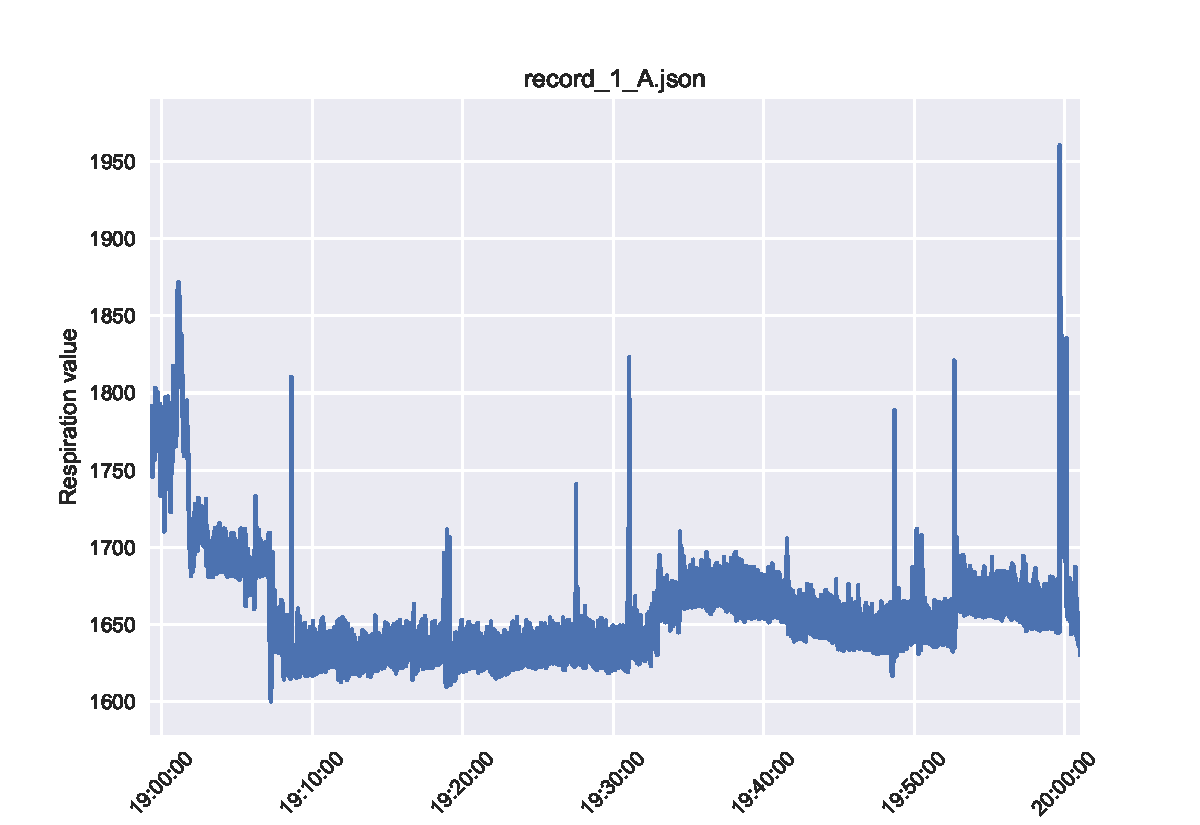
\includegraphics[scale=0.6]{images/record_1_a.pdf}
    \caption{Concert Day 1: Device A}
    \label{fig:concert_day1_a}
\end{figure}

\begin{figure}
    \centering
    \includegraphics[scale=0.6]{images/record_1_b.pdf}
    \caption{Concert Day 1: Device B}
    \label{fig:concert_day1_b}
\end{figure}

\begin{figure}
    \centering
    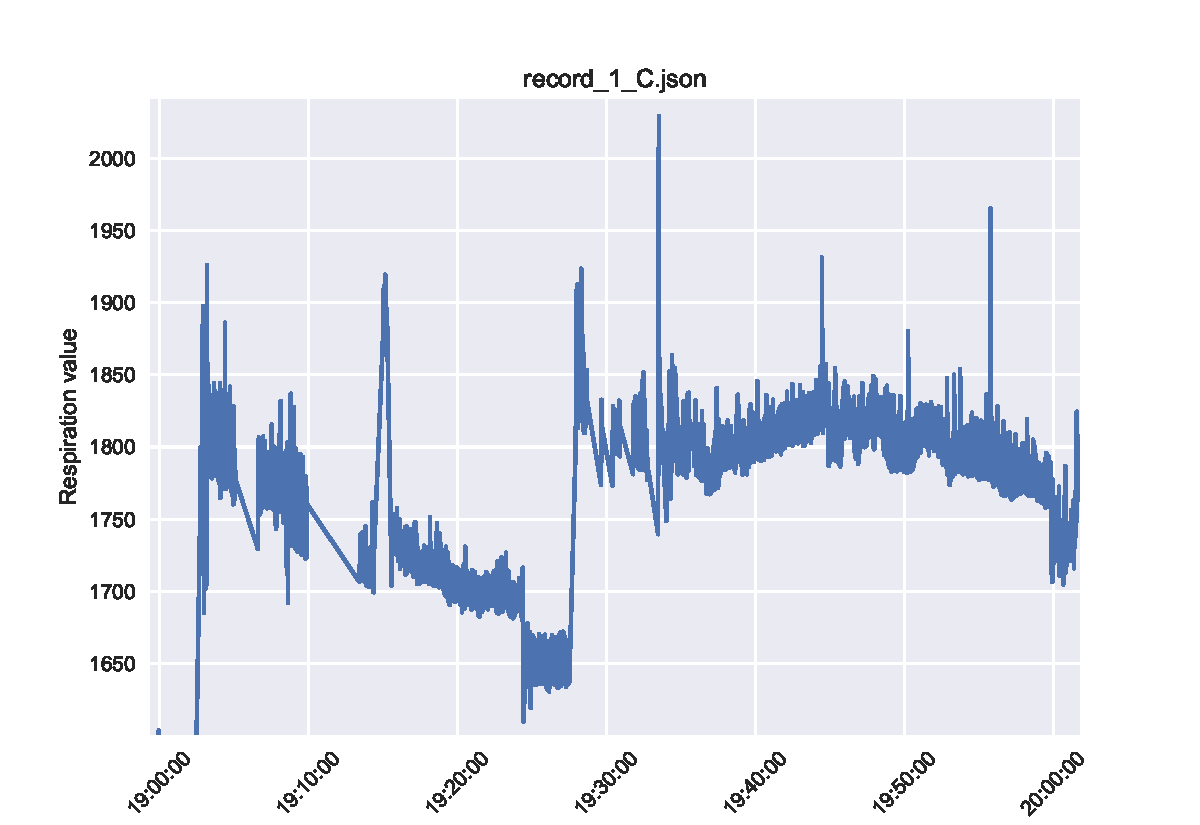
\includegraphics[scale=0.6]{images/record_1_c.pdf}
    \caption{Concert Day 1: Device C}
    \label{fig:concert_day1_c}
\end{figure}

\begin{figure}
    \centering
    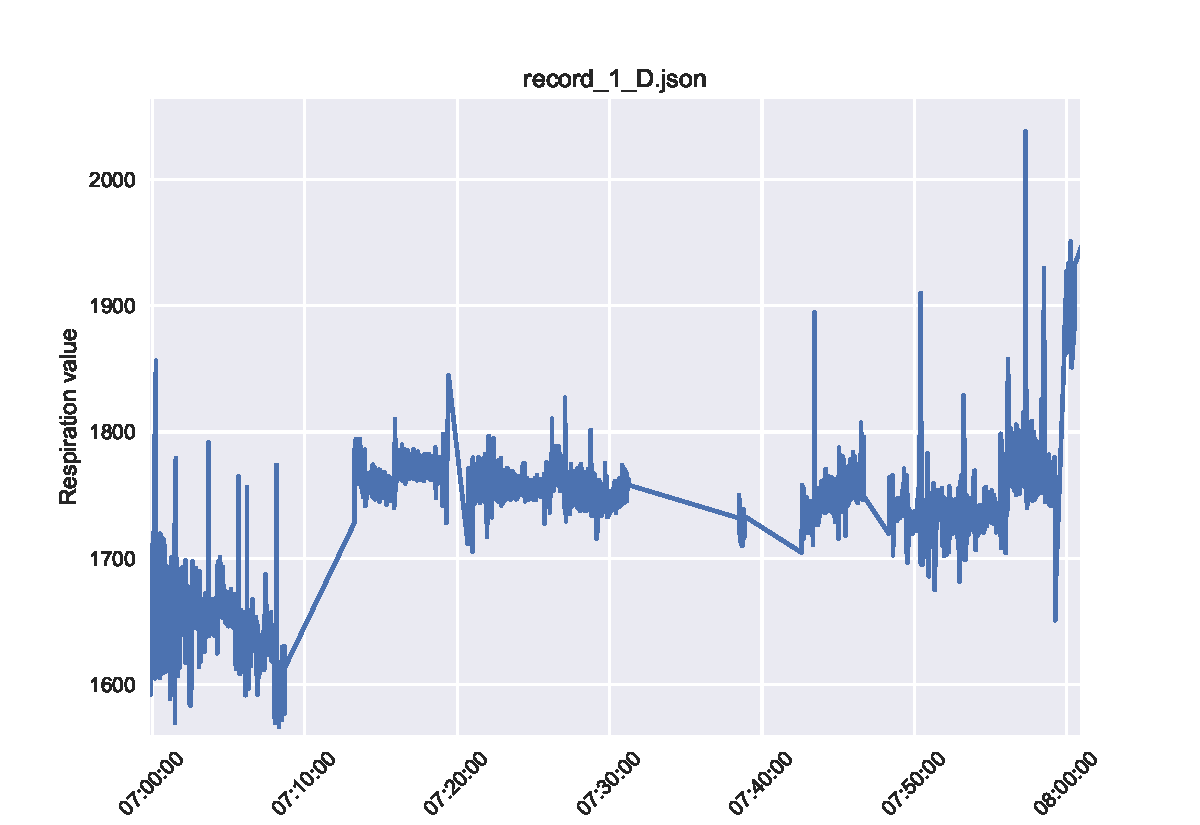
\includegraphics[scale=0.6]{images/record_1_d.pdf}
    \caption{Concert Day 1: Device D}
    \label{fig:concert_day1_d}
\end{figure}

\begin{figure}
    \centering
    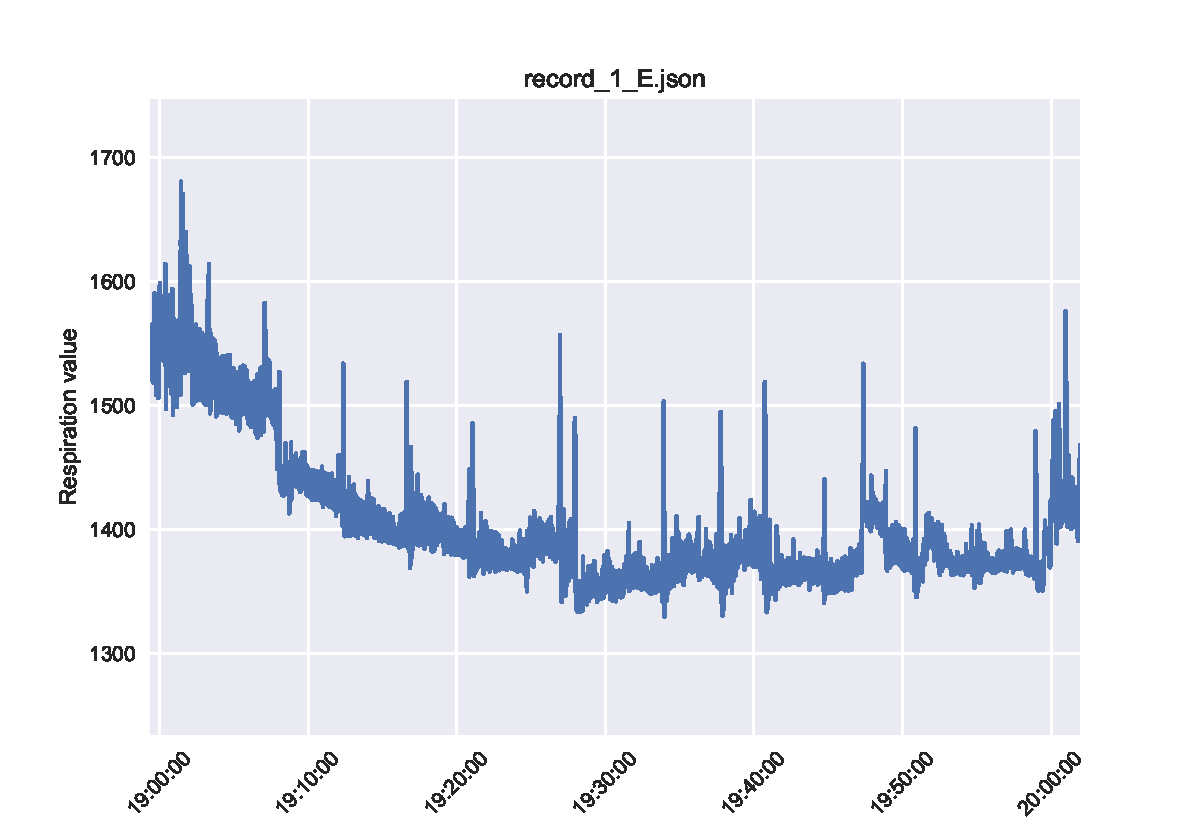
\includegraphics[scale=0.6]{images/record_1_e.pdf}
    \caption{Concert Day 1: Device E}
    \label{fig:concert_day1_e}
\end{figure}

\begin{figure}
    \centering
    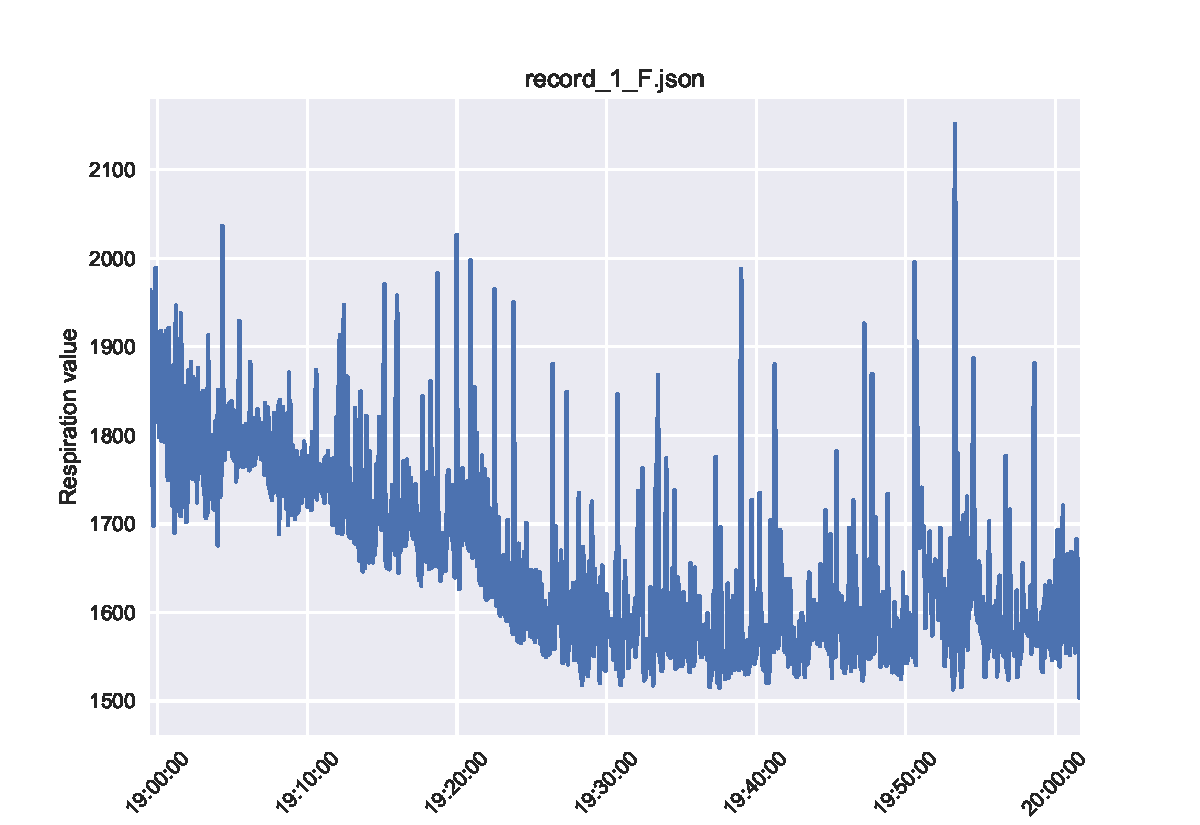
\includegraphics[scale=0.6]{images/record_1_f.pdf}
    \caption{Concert Day 1: Device F}
    \label{fig:concert_day1_f}
\end{figure}

\section{Concert Day 2: Time-Series Graph}


\begin{figure}
    \centering
    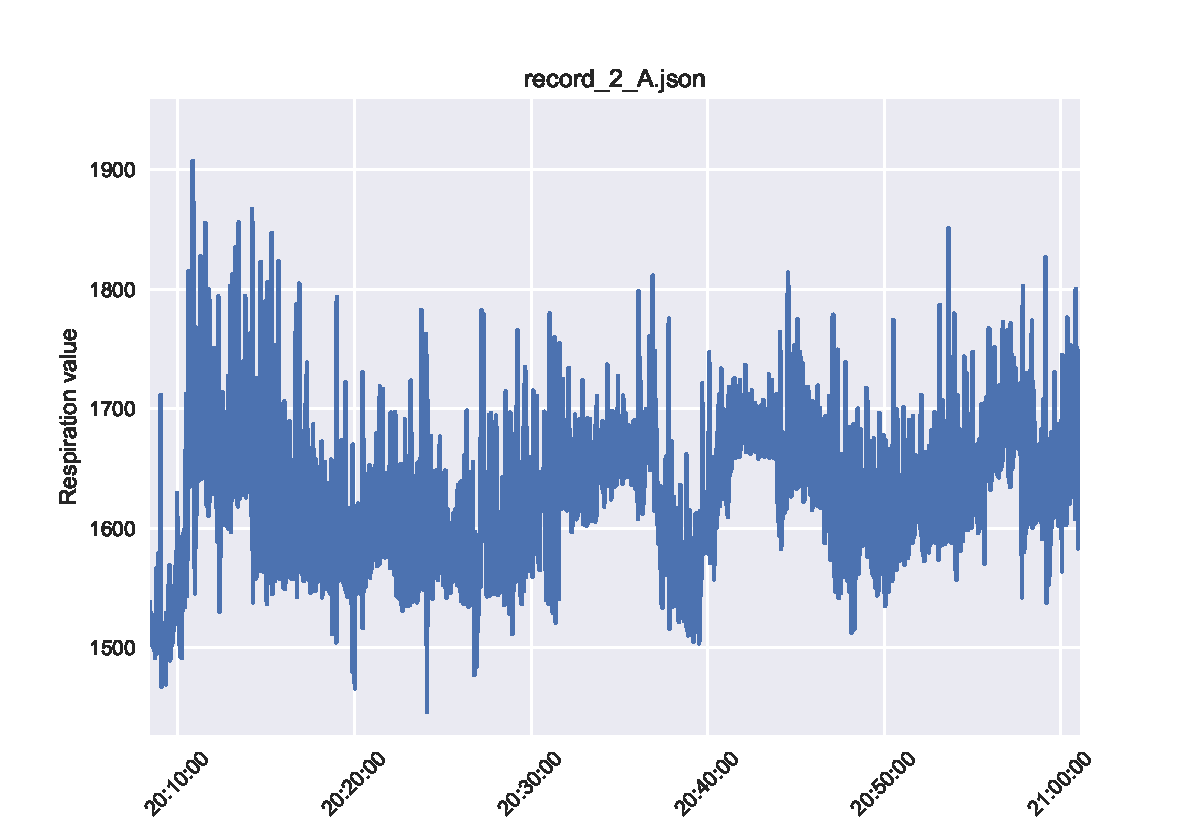
\includegraphics[scale=0.6]{images/record_2_a.pdf}
    \caption{Concert Day 2: Device A}
    \label{fig:concert_day2_a}
\end{figure}

\begin{figure}
    \centering
    \includegraphics[scale=0.6]{images/record_2_b.pdf}
    \caption{Concert Day 2: Device B}
    \label{fig:concert_day2_b}
\end{figure}

\begin{figure}
    \centering
    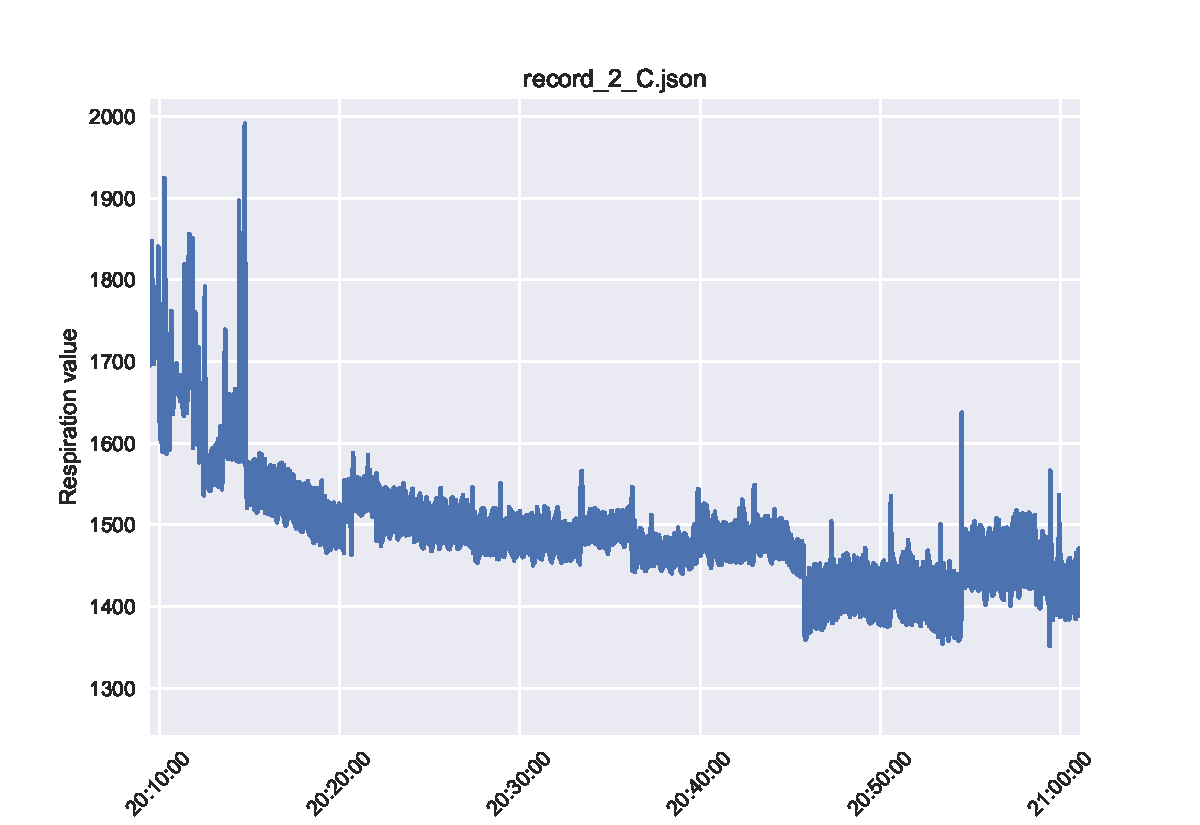
\includegraphics[scale=0.6]{images/record_2_c.pdf}
    \caption{Concert Day 2: Device C}
    \label{fig:concert_day2_c}
\end{figure}

\begin{figure}
    \centering
    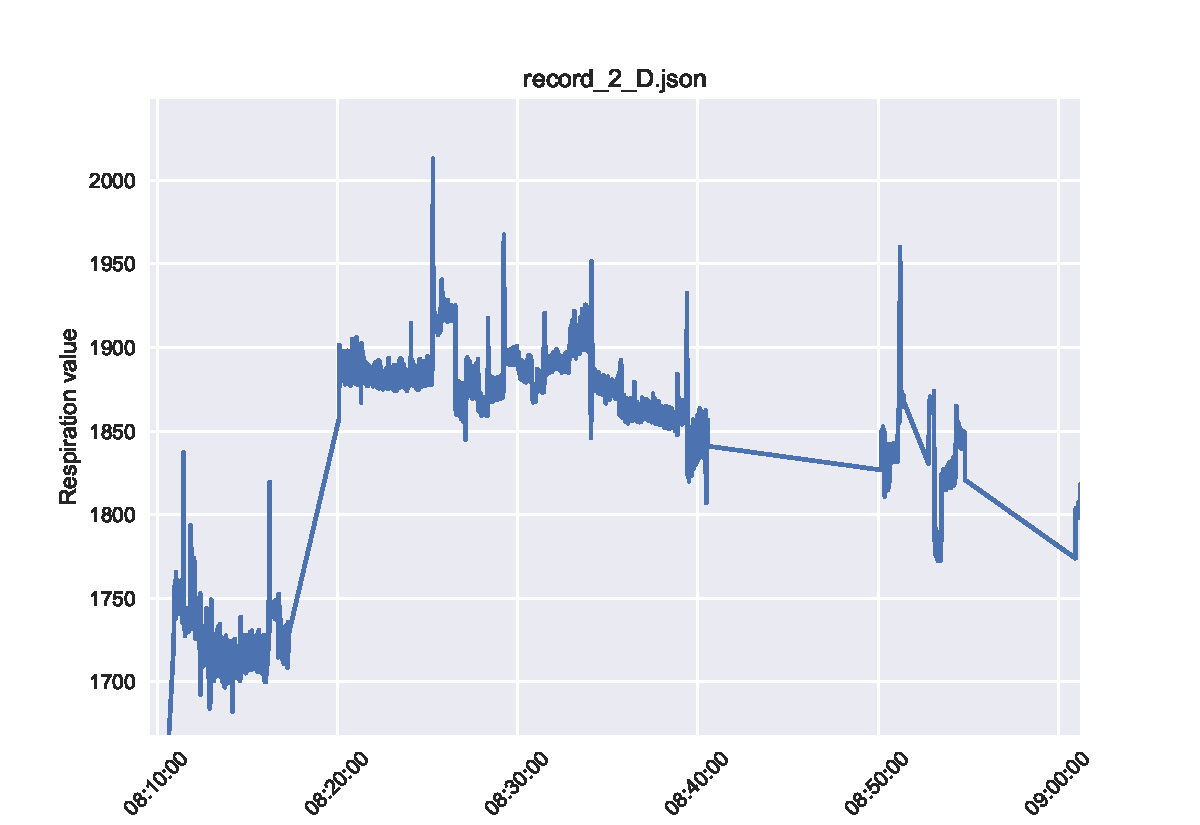
\includegraphics[scale=0.6]{images/record_2_d.pdf}
    \caption{Concert Day 2: Device D}
    \label{fig:concert_day2_d}
\end{figure}

\begin{figure}
    \centering
    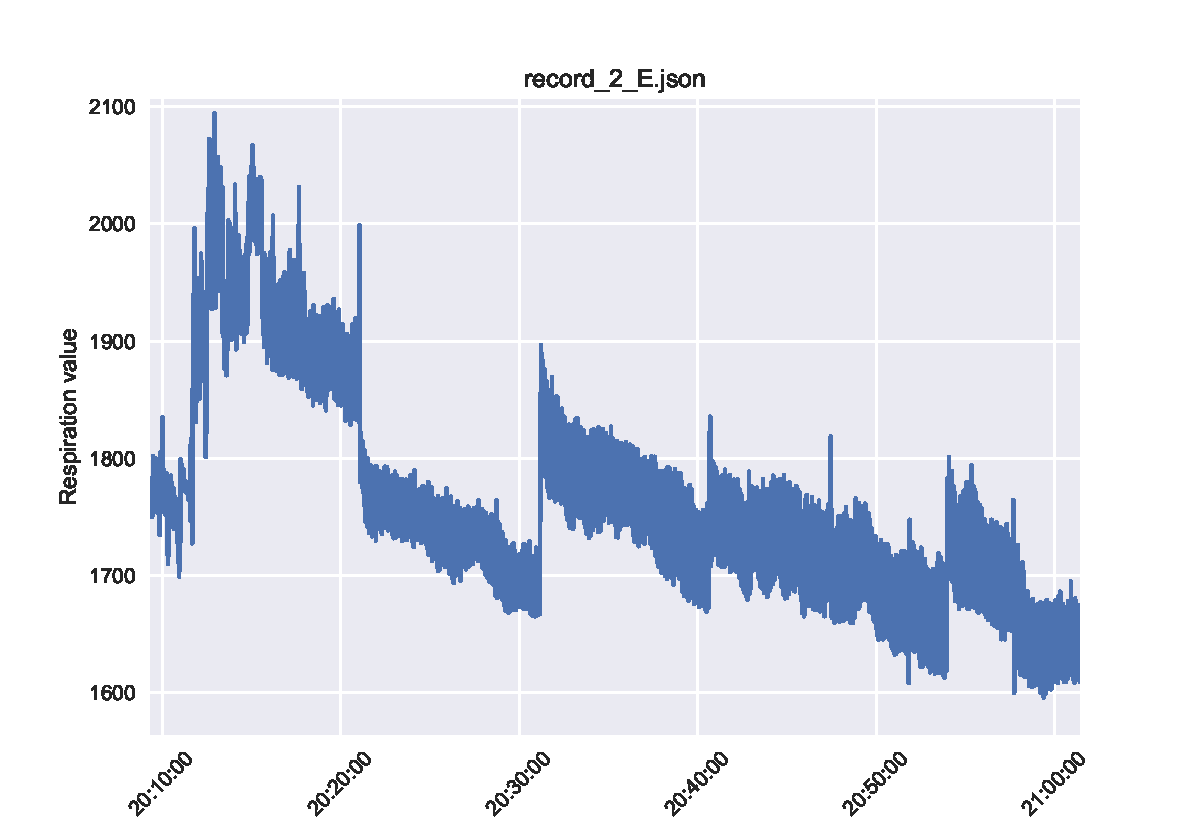
\includegraphics[scale=0.6]{images/record_2_e.pdf}
    \caption{Concert Day 2: Device E}
    \label{fig:concert_day2_e}
\end{figure}

\begin{figure}
    \centering
    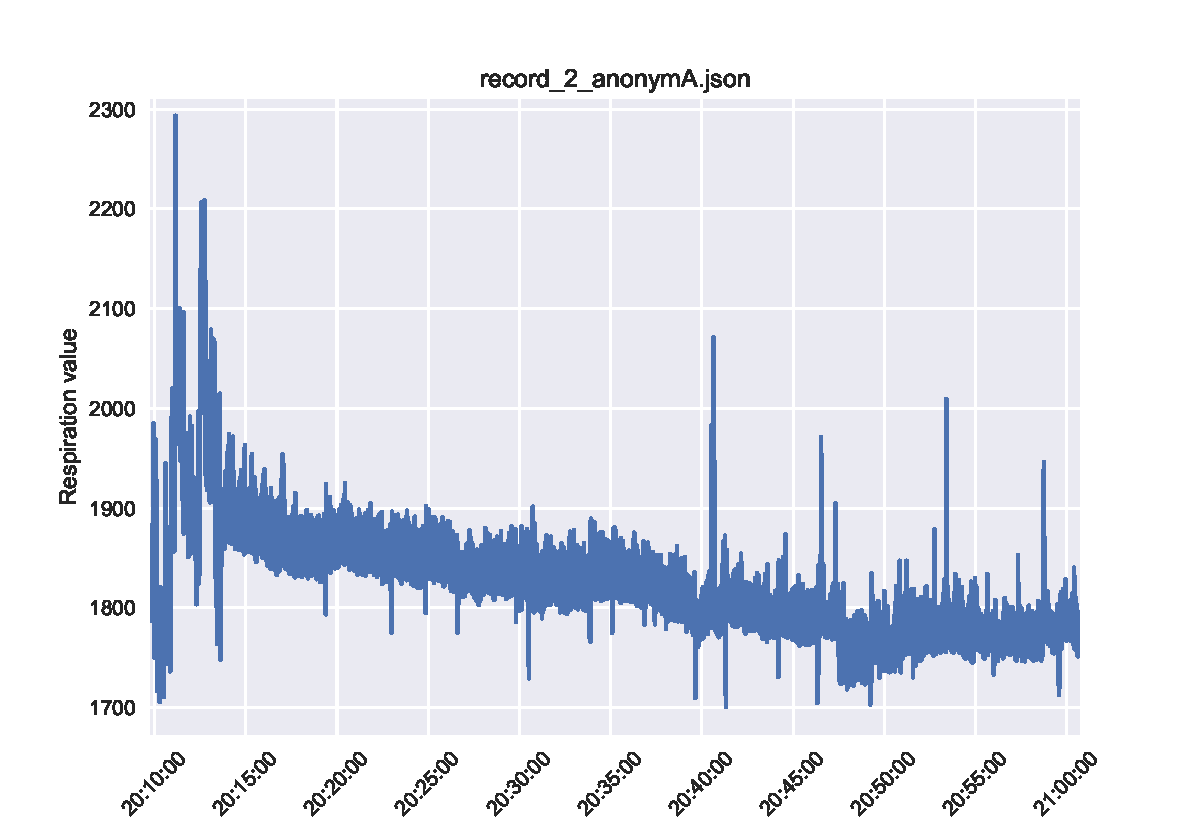
\includegraphics[scale=0.6]{images/record_2_f.pdf}
    \caption{Concert Day 2: Device F}
    \label{fig:concert_day2_f}
\end{figure}


\section{Python Code for Plotting}
The following Listing presents the code used for plotting the data from the concert into a time-series graph. 

\begin{lstlisting}[language=json, caption={My Caption}, captionpos=b]
import json
import matplotlib.pyplot as plt
from matplotlib.dates import DateFormatter
from datetime import datetime
from statistics import mean
import sys 
import seaborn

plt.style.use('seaborn')

sample_count = 0

def get_data(sample):
    data = sample[2].split("=")[1].split(",")
    avg = mean([int(i) for i in data])
    return avg

def get_date(sample):
    global sample_count

    if sample > '20:10:00' and sample < '21:00:00':
        sample_count += 1

    return datetime.strptime(sample, '%H:%M:%S')

def parse(data, name):
    global sample_count

    date = [get_date(i['implicitTS'].split(" ")[-1]) for i in data[0]['samples']]
    data = [get_data(i['sample'].split(", ")) for i in data[0]['samples']]

    fig, ax = plt.subplots()
    plt.plot(date, data)

    ax.xaxis.set_major_formatter(DateFormatter('%H:%M:%S'))
    ax.xaxis_date()
    ax.xaxis.set_tick_params(rotation=45)

    ax.set_xlabel("Time")
    ax.set_ylabel("Respiration value")
    ax.set_title(name)

    plt.show()
    
    print(sample_count)

def read(filename="record_1_B.json"):
    with open(filename) as f:
        json_data = json.load(f)

        parse(json_data, filename)

if __name__ == "__main__":
    if len(sys.argv) == 2:
        read(sys.argv[1])
    else:
        read()
\end{lstlisting}


\chapter{Module Pre-Code}